% Compile from repository root with:
% tectonic professor-report-final.tex
\documentclass[11pt,a4paper]{article}

\usepackage[utf8]{inputenc}
\usepackage[T1]{fontenc}
\usepackage[italian]{babel}
\usepackage{geometry}
\usepackage{graphicx}
\usepackage{booktabs}
\usepackage{array}
\usepackage{longtable}
\usepackage{float}
\usepackage{xcolor}
\usepackage{amsmath}
\usepackage{xurl}
\usepackage{hyperref}

\geometry{margin=2.1cm}
\hypersetup{
  colorlinks=true,
  linkcolor=blue,
  urlcolor=blue,
  citecolor=blue
}

\newcommand{\normal}{\textit{Normal}}
\newcommand{\pneumonia}{\textit{Pneumonia}}
\newcommand{\balacc}{balanced accuracy}
\newcommand{\auc}{ROC-AUC}
\newcommand{\githuburl}{\url{https://github.com/yahiag04/pneumonia-xray-classifier}}

\title{\textbf{Classificazione binaria di polmonite da radiografie toraciche -- Inquadramento per tesi}\\
\large Confronto tra reti CNN, generalizzazione cross-dataset e analisi statistica}
\author{Yahia Ghallale\\
\small Repository GitHub: \githuburl}
\date{Università degli Studi di Brescia \\ 1 luglio 2026}

\begin{document}
\maketitle

\begin{abstract}
Questo documento riassume lo stato finale degli esperimenti svolti finora per
la tesi sulla classificazione binaria \normal/\pneumonia{} da radiografie
toraciche. Il lavoro e' stato riorientato verso un setting adulto: il training
principale e' stato effettuato su un sottoinsieme binario e bilanciato del
dataset RSNA Pneumonia Detection Challenge, mentre le prestazioni sono state
misurate su test interno RSNA e su due dataset esterni, Kermany e Chittagong.
Sono state confrontate cinque reti: una CNN custom, denominata PneumoniaNet, e
quattro architetture note, ResNet18, MobileNetV3-Large, EfficientNet-B0 e
DenseNet121. In aggiunta sono stati eseguiti test zero-shot con modelli
TorchXRayVision pre-addestrati su dataset radiografici. L'analisi finale mostra
che non esiste una rete migliore in modo uniforme su tutti i dataset:
EfficientNet-B0 e' la migliore sul test interno RSNA, DenseNet121 e' la piu'
forte su Kermany, mentre su Chittagong PneumoniaNet rientra nel gruppo di testa
ma e' statisticamente indistinguibile da ResNet18, MobileNetV3-Large ed
EfficientNet-B0. E' stata inoltre aggiunta una prima estensione multi-classe
RSNA, in cui la classe esclusa \texttt{No Lung Opacity / Not Normal} viene
trattata come terza categoria distinta.
\end{abstract}

\tableofcontents
\newpage

\section{Obiettivo}

L'obiettivo della tesi e' valutare modelli di deep learning per la
classificazione binaria di radiografie toraciche in due classi:
\normal{} e \pneumonia. Il punto centrale non e' soltanto ottenere una buona
accuracy su un dataset, ma capire quanto le reti generalizzino quando vengono
testate su distribuzioni diverse.

La domanda sperimentale finale e':

\begin{quote}
\textit{Una rete addestrata in modo controllato su un dataset adulto e
pneumonia-specifico mantiene prestazioni robuste su dataset esterni? E una
singola architettura risulta migliore in modo stabile su tutti i domini?}
\end{quote}

Per rispondere sono stati separati due tipi di esperimento:

\begin{itemize}
  \item \textbf{zero-shot}: modelli gia' pre-addestrati su radiografie
  toraciche vengono valutati senza ulteriore training sui dataset esterni;
  \item \textbf{post-training}: le reti del progetto vengono addestrate sul
  training set RSNA adult-oriented e poi valutate su RSNA, Kermany e Chittagong.
\end{itemize}

\section{Dataset}

\subsection{RSNA adult-oriented}

Il dataset principale e' RSNA Pneumonia Detection Challenge
\cite{rsna_kaggle}. La scelta e' motivata dal fatto che il task e'
pneumonia-specifico e che la classe positiva deriva da annotazioni radiologiche
di opacita' polmonare, non da una semplice binarizzazione di un dataset
multi-label. La versione locale usata negli esperimenti contiene immagini PNG
processate e metadata compatibili con la preparazione binaria.

Per ottenere un task coerente con \normal/\pneumonia{} e' stata usata la
seguente mappatura:

\begin{itemize}
  \item \texttt{Normal} $\rightarrow$ \normal;
  \item \texttt{Lung Opacity} $\rightarrow$ \pneumonia;
  \item \texttt{No Lung Opacity / Not Normal} esclusa dal task binario.
\end{itemize}

E' stato costruito un subset bilanciato da 7000 immagini: 5000 per training,
1000 per validation e 1000 per test. Lo split e' stato fatto a livello di
\texttt{patientId}: prima dello split e' stata mantenuta una sola immagine per
paziente e poi i pazienti sono stati divisi tra training, validation e test.
Nel metadata finale ci sono 7000 righe e 7000 \texttt{patientId} unici; le
intersezioni train/validation, train/test e validation/test sono tutte nulle.
Questo evita leakage interno tra gli split RSNA.

I metadata RSNA includono anche la proiezione radiografica. Nel subset finale
sono presenti 3635 immagini PA e 3365 AP. La distribuzione per split e':
training 2621 PA e 2379 AP, validation 493 PA e 507 AP, test 521 PA e 479 AP.
I dataset esterni non hanno nel manifest locale lo stesso livello di metadata
DICOM; la view position rimane quindi un possibile confondente non completamente
controllabile nella valutazione cross-dataset.

Come estensione esplorativa e' stato poi costruito anche un task RSNA
multi-classe a tre classi, mantenendo la classe precedentemente esclusa:

\begin{itemize}
  \item \texttt{Normal} $\rightarrow$ \texttt{normal};
  \item \texttt{Lung Opacity} $\rightarrow$ \texttt{lung\_opacity};
  \item \texttt{No Lung Opacity / Not Normal} $\rightarrow$
  \texttt{not\_normal\_no\_lung\_opacity}.
\end{itemize}

Lo split multi-classe e' bilanciato a livello di classe: 2500 immagini per
classe in training, 500 per classe in validation e 500 per classe in test. Il
test multi-classe contiene quindi 1500 immagini totali, equamente divise tra le
tre categorie. Questa tabella descrive lo split disponibile; l'esperimento
multi-classe riportato piu' avanti non usa ancora il training set come
fine-tuning end-to-end completo, ma come linear probe sui checkpoint binari.

\subsection{Dataset esterni}

Sono stati usati due dataset esterni:

\begin{itemize}
  \item \textbf{Kermany}: dataset collegato allo studio di Kermany et al.
  \cite{kermany2018}. E' utile come test fuori distribuzione, ma non viene
  trattato come training principale perche' nasce da una popolazione pediatrica
  diversa dal target adult-oriented della tesi.
  \item \textbf{Chittagong}: dataset esterno indipendente con classi
  \normal{} e \pneumonia. E' stato usato solo lo split di test, senza
  fine-tuning, per misurare la generalizzazione esterna.
\end{itemize}

\begin{table}[H]
\centering
\caption{Dataset usati negli esperimenti finali.}
\begin{tabular}{lrrr}
\toprule
Dataset & Normal & Pneumonia & Totale \\
\midrule
RSNA train+val+test & 3500 & 3500 & 7000 \\
RSNA test & 500 & 500 & 1000 \\
Kermany test & 234 & 390 & 624 \\
Chittagong test & 257 & 256 & 513 \\
\bottomrule
\end{tabular}
\end{table}

\begin{table}[H]
\centering
\caption{Split RSNA multi-classe usato nell'estensione esplorativa.}
\begin{tabular}{lrrrr}
\toprule
Split & Normal & Lung opacity & Not normal/no opacity & Totale \\
\midrule
Train & 2500 & 2500 & 2500 & 7500 \\
Validation & 500 & 500 & 500 & 1500 \\
Test & 500 & 500 & 500 & 1500 \\
\bottomrule
\end{tabular}
\end{table}

\section{Modelli confrontati}

\subsection{PneumoniaNet}

PneumoniaNet e' la rete custom del progetto. E' una CNN compatta, pensata come
baseline controllata rispetto ad architetture piu' grandi pre-addestrate su
ImageNet. Lavora su input in scala di grigi e contiene circa 300 mila
parametri, quindi e' molto piu' piccola delle reti di confronto.

\begin{table}[H]
\centering
\caption{Struttura di PneumoniaNet.}
\begin{tabular}{lll}
\toprule
Blocco & Operazioni principali & Canali \\
\midrule
Input & radiografia 224x224 in scala di grigi & 1 \\
Blocco 1 & Conv 3x3 + BatchNorm + ReLU + MaxPool & 16 \\
Blocco 2 & Conv 3x3 + BatchNorm + ReLU, due volte + MaxPool & 32 \\
Blocco 3 & Conv 3x3 + BatchNorm + ReLU, due volte + MaxPool & 64 \\
Blocco 4 & Conv 3x3 + BatchNorm + ReLU, due volte + MaxPool & 128 \\
Pooling & Adaptive average pooling & 128 \\
Classifier & Linear 128$\rightarrow$64 + ReLU + Dropout + Linear 64$\rightarrow$1 & 1 logit \\
\bottomrule
\end{tabular}
\end{table}

\subsection{Reti di confronto}

Le reti di confronto sono state scelte per coprire famiglie CNN note e
ampiamente usate:

\begin{itemize}
  \item \textbf{ResNet18}: architettura residuale, basata su connessioni skip
  che facilitano l'ottimizzazione di reti profonde \cite{he2016resnet};
  \item \textbf{MobileNetV3-Large}: architettura efficiente progettata con
  hardware-aware search e blocchi compatti \cite{howard2019mobilenetv3};
  \item \textbf{EfficientNet-B0}: architettura basata su compound scaling, cioe'
  bilanciamento congiunto di profondita', larghezza e risoluzione
  \cite{tan2019efficientnet};
  \item \textbf{DenseNet121}: architettura con connessioni dense tra layer, che
  favoriscono riuso delle feature e propagazione del gradiente
  \cite{huang2017densenet}.
\end{itemize}

\begin{table}[H]
\centering
\caption{Dimensione, costo computazionale e andamento del training su RSNA. Il GMAC e' calcolato per una inferenza con input 224x224 e conta le operazioni MAC di layer convoluzionali e lineari, in linea con analisi pratiche costo/accuratezza di reti neurali profonde \cite{canziani2016analysis}.}
\begin{tabular}{llrrrr}
\toprule
Modello & Input & Parametri & GMAC & Best epoch & Epoche eseguite \\
\midrule
PneumoniaNet & 1x224x224 & 300161 & 0.527 & 5 & 10 \\
ResNet18 & 3x224x224 & 11177025 & 1.814 & 10 & 15 \\
MobileNetV3-Large & 3x224x224 & 4203313 & 0.215 & 5 & 10 \\
EfficientNet-B0 & 3x224x224 & 4008829 & 0.385 & 4 & 9 \\
DenseNet121 & 3x224x224 & 6954881 & 2.833 & 6 & 11 \\
\bottomrule
\end{tabular}
\end{table}

La tabella separa due aspetti diversi della leggerezza di un modello.
PneumoniaNet e' nettamente la piu' piccola in termini di parametri, quindi ha
un costo di memoria inferiore rispetto alle architetture pre-addestrate. Non e'
pero' la piu' economica in termini di operazioni per inferenza: MobileNetV3-Large
ed EfficientNet-B0 hanno meno GMAC grazie a blocchi progettati esplicitamente
per efficienza computazionale. Di conseguenza la rete custom va descritta come
compatta in memoria, non come architettura computazionalmente ottimizzata.

\section{Metriche}

Per evitare conclusioni fuorvianti in presenza di dataset sbilanciati, la
metrica principale e' la \balacc:

\[
\text{Balanced Accuracy} =
\frac{\text{Sensitivity} + \text{Specificity}}{2}.
\]

Sono state inoltre riportate accuracy, sensitivity, specificity, ROC-AUC,
PR-AUC, F1-score e confusion matrix. Per la parte finale sono stati aggiunti:

\begin{itemize}
  \item \textbf{bootstrap confidence intervals}: intervalli al 95\% tramite
  bootstrap stratificato, ispirati al principio bootstrap di Efron
  \cite{efron1979bootstrap};
  \item \textbf{McNemar test}: test paired sulle predizioni corrette/errate di
  due classificatori sullo stesso dataset \cite{mcnemar1947};
  \item \textbf{DeLong test}: confronto statistico tra AUC correlate, quindi
  calcolate sugli stessi campioni \cite{delong1988};
  \item \textbf{Holm-Bonferroni}: correzione per confronti multipli applicata
  separatamente entro ciascun dataset e tipo di test, cosi' da non interpretare
  come stabile un risultato borderline dovuto al numero di confronti
  \cite{holm1979}.
\end{itemize}

\section{Esperimenti zero-shot}

Prima del training adult-oriented e' stato eseguito un esperimento economico:
valutare modelli TorchXRayVision gia' pre-addestrati su radiografie toraciche.
TorchXRayVision fornisce dataset, preprocessing e modelli pre-addestrati per
CXR, ed e' adatto come baseline esterna \cite{torchxrayvision}. Sono stati
usati tre DenseNet121:

\begin{itemize}
  \item \texttt{densenet121-res224-rsna};
  \item \texttt{densenet121-res224-nih};
  \item \texttt{densenet121-res224-all}.
\end{itemize}

\begin{table}[H]
\centering
\caption{Risultati zero-shot TorchXRayVision.}
\begin{tabular}{llrrr}
\toprule
Dataset & Modello zero-shot & \balacc & \auc & Sens./Spec. \\
\midrule
Kermany & DenseNet-RSNA & 0.668 & 0.825 & 0.944 / 0.393 \\
Kermany & DenseNet-NIH & 0.777 & 0.880 & 0.656 / 0.897 \\
Kermany & DenseNet-All & 0.582 & 0.791 & 0.172 / 0.991 \\
Chittagong & DenseNet-RSNA & 0.813 & 0.905 & 0.805 / 0.821 \\
Chittagong & DenseNet-NIH & 0.635 & 0.705 & 0.531 / 0.739 \\
Chittagong & DenseNet-All & 0.574 & 0.576 & 0.164 / 0.984 \\
\bottomrule
\end{tabular}
\end{table}

Il risultato piu' importante e' che su Chittagong il modello pre-addestrato su
RSNA e' nettamente superiore agli altri zero-shot. Questo supporta la scelta di
un training adult-oriented e pneumonia-specifico. Su Kermany invece il modello
NIH ha la \balacc{} piu' alta: questo conferma che il comportamento dipende dal
dataset e che le conclusioni non possono basarsi su un singolo test.

La stessa conclusione emerge confrontando, sullo stesso dataset Chittagong, le
reti addestrate nella fase iniziale su Kermany con le stesse architetture
addestrate successivamente su RSNA. Il passaggio a RSNA migliora la \balacc{}
media da circa 0.636 a circa 0.801, con un incremento medio di circa 0.165. Con
solo cinque architetture, questo confronto va letto come descrittivo: i delta
vanno da +0.082 a +0.211 e non costituiscono un intervallo inferenziale robusto.

\begin{table}[H]
\centering
\caption{Confronto su Chittagong: training iniziale su Kermany vs training su RSNA.}
\begin{tabular}{lrrr}
\toprule
Modello & Kermany$\rightarrow$Chittagong BA & RSNA$\rightarrow$Chittagong BA & Delta \\
\midrule
PneumoniaNet & 0.634 & 0.830 & +0.196 \\
ResNet18 & 0.608 & 0.819 & +0.211 \\
MobileNetV3 & 0.618 & 0.797 & +0.179 \\
EfficientNet-B0 & 0.636 & 0.795 & +0.159 \\
DenseNet121 & 0.682 & 0.764 & +0.082 \\
\midrule
Media & 0.636 & 0.801 & +0.165 \\
\bottomrule
\end{tabular}
\end{table}

Questo e' il motivo empirico principale per non usare Kermany come dataset di
training finale: a parita' di architettura, il training su RSNA trasferisce
meglio su Chittagong.

\section{Esperimenti post-training su RSNA}

Tutte le reti sono state addestrate sullo stesso subset RSNA bilanciato, con
early stopping e soglia decisionale 0.5. La tabella seguente riporta i risultati
principali con intervalli bootstrap al 95\%.

\small
\begin{longtable}{llrrrlrl}
\caption{Benchmark post-training. BA = balanced accuracy.}\label{tab:benchmark-post-training}\\
\toprule
Dataset & Modello & Sens. & Spec. & BA & BA 95\% CI & \auc & AUC 95\% CI \\
\midrule
\endfirsthead
\toprule
Dataset & Modello & Sens. & Spec. & BA & BA 95\% CI & \auc & AUC 95\% CI \\
\midrule
\endhead
RSNA & PneumoniaNet & 0.918 & 0.874 & 0.896 & [0.877, 0.914] & 0.961 & [0.949, 0.971] \\
RSNA & ResNet18 & 0.956 & 0.926 & 0.941 & [0.926, 0.956] & 0.989 & [0.983, 0.993] \\
RSNA & MobileNetV3 & 0.942 & 0.946 & 0.944 & [0.929, 0.956] & 0.990 & [0.985, 0.993] \\
RSNA & EfficientNet-B0 & 0.944 & 0.956 & \textbf{0.950} & [0.935, 0.962] & 0.989 & [0.983, 0.993] \\
RSNA & DenseNet121 & 0.936 & 0.948 & 0.942 & [0.927, 0.956] & 0.987 & [0.981, 0.992] \\
\midrule
Kermany & PneumoniaNet & 0.944 & 0.432 & 0.688 & [0.654, 0.724] & 0.789 & [0.750, 0.825] \\
Kermany & ResNet18 & 0.956 & 0.487 & 0.722 & [0.685, 0.756] & 0.854 & [0.821, 0.884] \\
Kermany & MobileNetV3 & 0.895 & 0.679 & 0.787 & [0.754, 0.820] & 0.874 & [0.845, 0.901] \\
Kermany & EfficientNet-B0 & 0.867 & 0.769 & 0.818 & [0.786, 0.847] & 0.903 & [0.877, 0.925] \\
Kermany & DenseNet121 & 0.849 & 0.868 & \textbf{0.858} & [0.831, 0.884] & \textbf{0.925} & [0.903, 0.944] \\
\midrule
Chittagong & PneumoniaNet & 0.875 & 0.786 & \textbf{0.830} & [0.795, 0.864] & 0.887 & [0.854, 0.915] \\
Chittagong & ResNet18 & 0.816 & 0.821 & 0.819 & [0.784, 0.852] & 0.893 & [0.861, 0.921] \\
Chittagong & MobileNetV3 & 0.707 & 0.887 & 0.797 & [0.762, 0.832] & \textbf{0.904} & [0.878, 0.930] \\
Chittagong & EfficientNet-B0 & 0.668 & 0.922 & 0.795 & [0.758, 0.828] & 0.894 & [0.863, 0.922] \\
Chittagong & DenseNet121 & 0.602 & 0.926 & 0.764 & [0.729, 0.797] & 0.844 & [0.807, 0.878] \\
\bottomrule
\end{longtable}
\normalsize

\begin{table}[H]
\centering
\caption{Rapporto tra \balacc{} e costo computazionale. Valori piu' alti indicano piu' \balacc{} per GMAC, ma non sostituiscono le metriche cliniche principali.}
\begin{tabular}{lrrr}
\toprule
Modello & RSNA BA/GMAC & Kermany BA/GMAC & Chittagong BA/GMAC \\
\midrule
PneumoniaNet & 1.70 & 1.30 & 1.57 \\
ResNet18 & 0.52 & 0.40 & 0.45 \\
MobileNetV3-Large & 4.39 & 3.66 & 3.70 \\
EfficientNet-B0 & 2.47 & 2.13 & 2.07 \\
DenseNet121 & 0.33 & 0.30 & 0.27 \\
\bottomrule
\end{tabular}
\end{table}

Questa lettura costo/prestazione, usata qui come indicatore interno e non come
metrica clinica, mostra che l'aumento di capacita' non produce
un miglioramento proporzionale all'aumento del costo computazionale. Su RSNA,
EfficientNet-B0 ottiene la \balacc{} piu' alta, ma MobileNetV3-Large ha il
miglior rapporto BA/GMAC. Su Kermany DenseNet121 rimane il modello piu'
accurato, ma e' anche il piu' costoso; EfficientNet-B0 e MobileNetV3-Large
offrono un compromesso piu' favorevole tra prestazioni e costo. Su Chittagong
PneumoniaNet e' competitiva in \balacc{}, mentre MobileNetV3-Large resta la
scelta piu' efficiente se si considera il numero di operazioni.

\section{Studio di scaling controllato}

Per isolare l'effetto della capacita' del modello e' stato aggiunto uno studio
di scaling controllato sullo stesso task binario RSNA. L'obiettivo non e'
scegliere un nuovo modello finale, ma misurare quanta capacita' serve per
avvicinarsi alla top-performance mantenendo invariati dataset, seed,
augmentation, soglia 0.5, early stopping e loop di training. La sola variabile
sperimentale e' la complessita' dell'architettura.

Sono state costruite due curve:

\begin{itemize}
  \item \textbf{PneumoniaNet continua}: la rete custom e' stata resa parametrica
  con un moltiplicatore di larghezza \(w\). I canali base
  \(16,32,64,128\) e la testa fully-connected vengono scalati da \(w\).
  Il caso \(w=1.0\) riproduce esattamente la rete originale e mantiene
  300161 parametri.
  \item \textbf{EfficientNet discreta}: sono state addestrate le varianti
  ufficiali ImageNet-pretrained B0, B1, B2 e B3, senza modificare la struttura
  interna delle architetture.
\end{itemize}

La dimensione del training set e' stata resa parametrica nello script
\path{scripts/run_scaling_study.py}; nel risultato riportato qui e' stato usato
il subset RSNA corrente, cioe' 2500 immagini normali e 2500 immagini con
opacita' nel training set. Questa scelta rende il confronto direttamente
comparabile con gli esperimenti principali.

Va distinta la confrontabilita' di protocollo dalla confrontabilita' di
checkpoint. Il punto PneumoniaNet \(w=1.0\) ha la stessa architettura della
PneumoniaNet del benchmark principale, ma e' una nuova run di training dello
studio di scaling, non lo stesso checkpoint riportato nella tabella benchmark.
Infatti il benchmark principale seleziona il best checkpoint a epoca 5, mentre
la run di scaling \(w=1.0\) seleziona il best checkpoint a epoca 16. Questo
spiega la discrepanza numerica tra la tabella benchmark e la tabella di scaling
per la stessa architettura: 0.896 contro 0.914 su RSNA e 0.830 contro 0.756 su
Chittagong. Per EfficientNet-B0, invece, la ripetizione con lo stesso seed ha
prodotto lo stesso \texttt{model\_state} del benchmark principale, quindi le
metriche coincidono. I valori assoluti delle due tabelle non devono quindi
essere usati come se tutti i punti fossero la stessa identica esecuzione; il
seed controllato rende il protocollo riproducibile, ma non garantisce la stessa
traiettoria per ogni architettura e backend. La tabella di scaling serve
soprattutto a leggere l'andamento interno delle curve addestrate o riprodotte
nello stesso protocollo.

\begin{table}[H]
\centering
\caption{Scaling continuo di PneumoniaNet. BA = balanced accuracy.}
\small
\begin{tabular}{lrrrrr}
\toprule
Width & Parametri & GMAC & RSNA BA & Kermany BA & Chittagong BA \\
\midrule
0.5 & 75457 & 0.134 & 0.922 & 0.716 & 0.815 \\
1.0 & 300161 & 0.527 & 0.914 & 0.686 & 0.756 \\
1.5 & 674113 & 1.181 & 0.922 & 0.722 & 0.780 \\
2.0 & 1197313 & 2.095 & 0.922 & 0.666 & 0.807 \\
3.0 & 2691457 & 4.704 & \textbf{0.924} & 0.677 & \textbf{0.817} \\
4.0 & 4782593 & 8.353 & 0.923 & \textbf{0.724} & 0.795 \\
\bottomrule
\end{tabular}
\normalsize
\end{table}

\begin{table}[H]
\centering
\caption{Scaling discreto EfficientNet. Le varianti sono inizializzate da pesi ImageNet ufficiali. BA = balanced accuracy.}
\small
\begin{tabular}{lrrrrr}
\toprule
Variante & Parametri & GMAC & RSNA BA & Kermany BA & Chittagong BA \\
\midrule
B0 & 4008829 & 0.385 & \textbf{0.950} & \textbf{0.818} & 0.795 \\
B1 & 6514465 & 0.568 & 0.946 & 0.733 & 0.674 \\
B2 & 7702403 & 0.658 & 0.947 & 0.780 & \textbf{0.805} \\
B3 & 10697769 & 0.961 & 0.936 & 0.805 & 0.750 \\
\bottomrule
\end{tabular}
\normalsize
\end{table}

\begin{figure}[H]
\centering
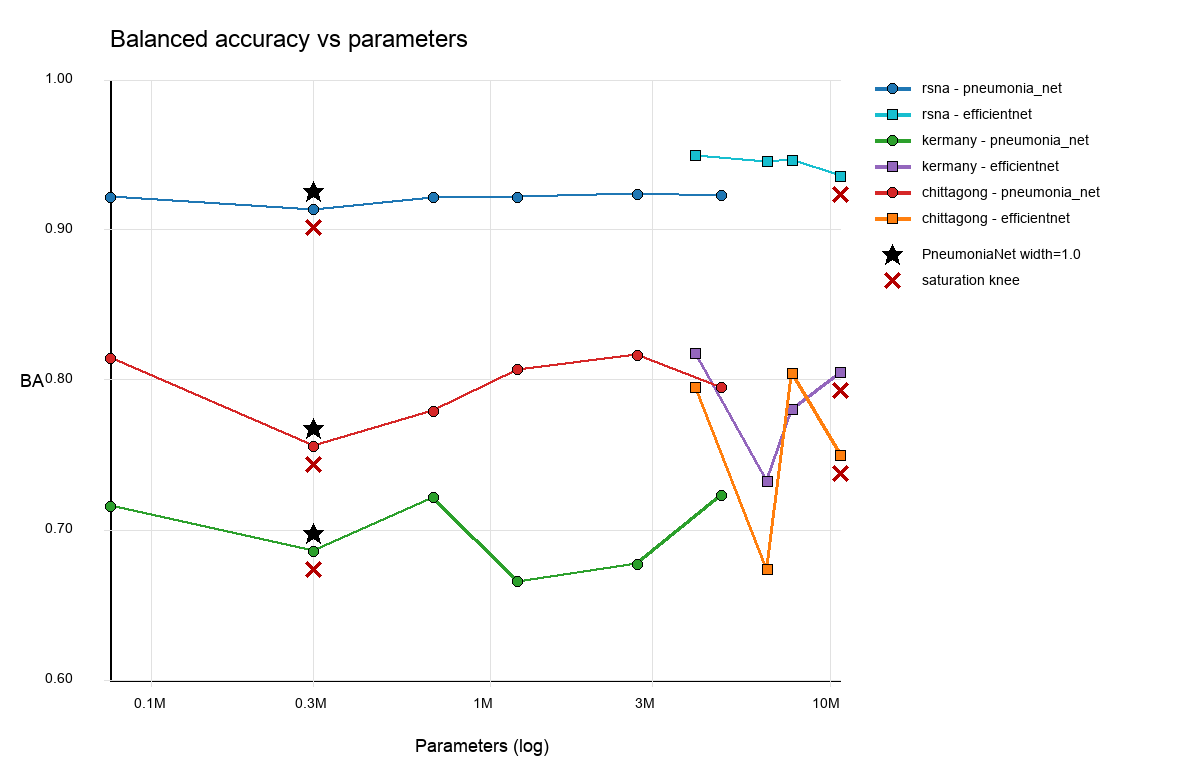
\includegraphics[width=0.92\linewidth]{outputs/scaling_study/balanced_accuracy_vs_params.png}
\caption{Studio di scaling: \balacc{} rispetto al numero di parametri, con asse x logaritmico. La stella indica PneumoniaNet \(w=1.0\); le croci indicano il ginocchio di saturazione stimato.}
\end{figure}

\begin{figure}[H]
\centering
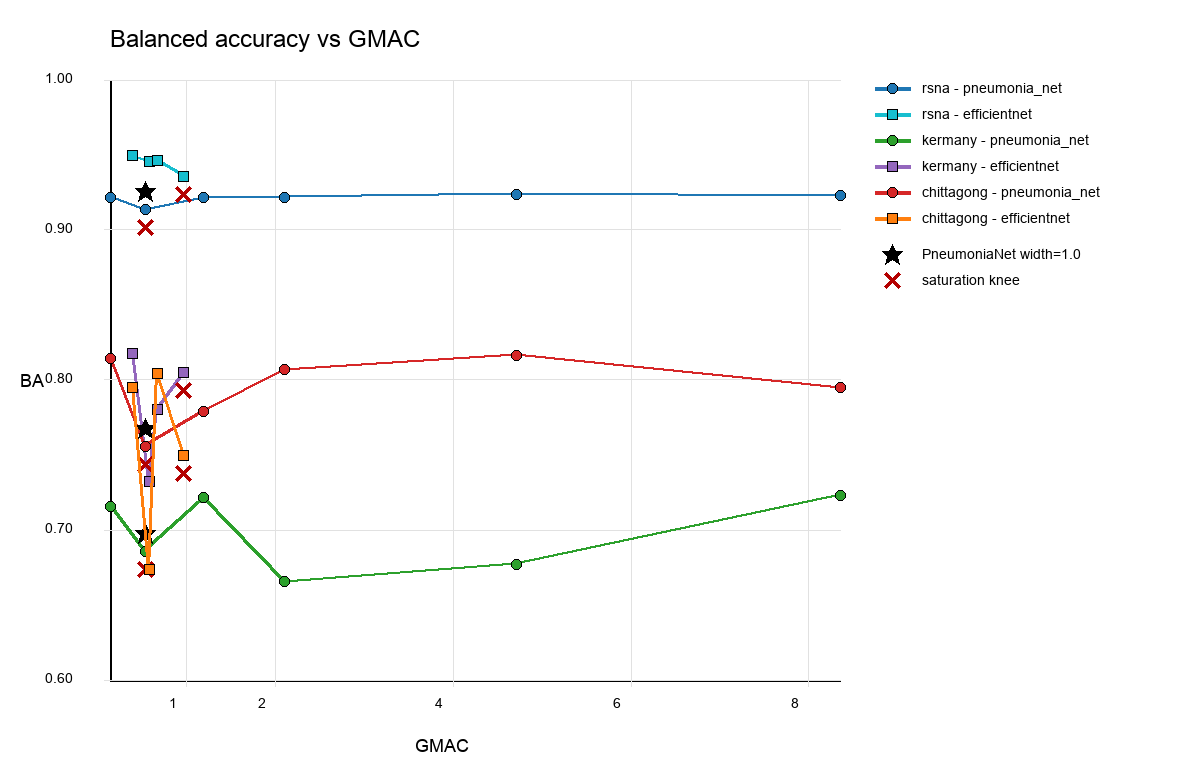
\includegraphics[width=0.92\linewidth]{outputs/scaling_study/balanced_accuracy_vs_gmac.png}
\caption{Studio di scaling: \balacc{} rispetto al costo computazionale in GMAC.}
\end{figure}

Il risultato piu' pulito riguarda RSNA interno. Per PneumoniaNet, passare da
75457 parametri a 4.78 milioni di parametri cambia la \balacc{} solo da 0.922 a
0.923, con massimo osservato 0.924 a \(w=3.0\). Anche nella famiglia
EfficientNet la curva non migliora con la dimensione: B0 ottiene 0.950, B1
0.946, B2 0.947 e B3 0.936. La performance interna satura quindi ben prima del
limite di capacita' esplorato, ma l'andamento va letto come piatto entro la
variabilita' del training piu' che come plateau monotono.

Sui dataset esterni, invece, le curve non sono monotone. PneumoniaNet oscilla da
0.666 a 0.724 su Kermany e da 0.756 a 0.817 su Chittagong. EfficientNet mostra
lo stesso problema: su Chittagong B1 scende a 0.674, mentre B0 e B2 sono vicine
a 0.80. Queste oscillazioni sono della stessa grandezza, o piu' grandi,
dell'effetto atteso della capacita'. Con un solo seed non e' quindi possibile
separare in modo affidabile l'effetto della complessita' dal rumore del training
sulla generalizzazione esterna. Lo studio mostra una curva interna quasi piatta,
ma non consente una conclusione forte sullo scaling esterno.

Operativamente, il prossimo passo non e' soltanto aumentare la capacita', ma
misurare la variabilita'. Lo stesso script permette di rilanciare lo studio con
piu' seed e con una dimensione del training set diversa tramite
\texttt{--train-size}. Solo una curva multi-seed, eventualmente ripetuta con
piu' immagini RSNA, puo' distinguere saturazione da capacita', saturazione da
dati e rumore stocastico del training.

\section{Estensione multi-classe RSNA}

Per rispondere all'ipotesi di aggiungere la terza classe esclusa finora, e'
stato preparato un task RSNA a tre classi:
\texttt{normal}, \texttt{lung\_opacity} e
\texttt{not\_normal\_no\_lung\_opacity}. Quest'ultima classe corrisponde alla
categoria RSNA esclusa dal task binario: radiografie non normali ma senza
opacita' polmonare annotata. L'estensione resta quindi coerente con
l'impostazione del progetto, che distingue presenza o assenza di opacita'
polmonare/polmonite e non introduce sottotipi eziologici.

Per rendere l'esperimento rapido e collegato al lavoro binario gia' svolto, ogni
modello e' stato inizializzato dal proprio checkpoint RSNA binario. Sono stati
caricati tutti i layer compatibili e sostituita la testa finale con una nuova
uscita a tre logit. Per le architetture pre-addestrate la backbone e' stata
congelata ed e' stata addestrata la testa multi-classe per una epoca; per
PneumoniaNet e' stato usato lo stesso checkpoint binario come inizializzazione.
Questa analisi e' quindi una prima stima del trasferimento dal task binario al
task a tre classi, coerente con l'idea che le feature apprese possano trasferire
in modo non uniforme tra task correlati \cite{yosinski2014transferable}, non
ancora un fine-tuning completo multi-classe.

\begin{table}[H]
\centering
\caption{Risultati preliminari sul task RSNA multi-classe. I modelli sono inizializzati dai rispettivi checkpoint binari RSNA. BA indica macro recall.}
\begin{tabular}{lrrrr}
\toprule
Modello & Accuracy & BA & Macro precision & Macro F1 \\
\midrule
PneumoniaNet & 0.507 & 0.507 & 0.526 & 0.471 \\
ResNet18 & 0.677 & 0.677 & 0.672 & 0.674 \\
MobileNetV3-Large & \textbf{0.692} & \textbf{0.692} & \textbf{0.677} & \textbf{0.677} \\
EfficientNet-B0 & 0.687 & 0.687 & 0.671 & 0.663 \\
DenseNet121 & 0.687 & 0.687 & 0.671 & 0.670 \\
\bottomrule
\end{tabular}
\end{table}

\begin{table}[H]
\centering
\caption{Recall per classe nel task RSNA multi-classe.}
\begin{tabular}{lrrr}
\toprule
Modello & Normal & Lung opacity & Not normal/no opacity \\
\midrule
PneumoniaNet & 0.924 & 0.370 & 0.228 \\
ResNet18 & 0.822 & 0.732 & \textbf{0.478} \\
MobileNetV3-Large & \textbf{0.900} & 0.764 & 0.412 \\
EfficientNet-B0 & 0.894 & \textbf{0.828} & 0.340 \\
DenseNet121 & 0.894 & 0.788 & 0.380 \\
\bottomrule
\end{tabular}
\end{table}

\begin{table}[H]
\centering
\caption{Confusion matrix multi-classe di MobileNetV3-Large su RSNA test, modello migliore per BA macro. Le righe sono le classi vere, le colonne le predizioni.}
\begin{tabular}{lrrr}
\toprule
Classe vera & Pred. normal & Pred. lung opacity & Pred. not normal \\
\midrule
Normal & 450 & 3 & 47 \\
Lung opacity & 17 & 382 & 101 \\
Not normal/no opacity & 121 & 173 & 206 \\
\bottomrule
\end{tabular}
\end{table}

Il risultato principale va letto come limite del trasferimento dal task binario
al task multi-classe. Le feature usate in questo protocollo sono state ottimizzate
per separare opacita' polmonare da assenza di opacita', mentre la classe
\texttt{not\_normal\_no\_lung\_opacity} non era presente nel training binario.
Le architetture pre-addestrate e poi adattate al task binario trasferiscono
meglio di PneumoniaNet al task a tre classi: MobileNetV3-Large ottiene la BA
macro piu' alta (0.692), seguita da EfficientNet-B0 e DenseNet121 (0.687) e
ResNet18 (0.677). Tuttavia nessun modello separa bene la terza classe con una
sola testa multi-classe: il miglior recall su
\texttt{not\_normal\_no\_lung\_opacity} e' 0.478 con ResNet18, mentre
MobileNetV3-Large raggiunge 0.412. La confusion matrix di MobileNetV3-Large
mostra che molti esempi della terza classe vengono proiettati sull'asse binario
gia' appreso e quindi assorbiti da \texttt{normal} o \texttt{lung\_opacity}.
L'esperimento va quindi letto come linear probe sui checkpoint binari, utile per
mostrare che un vero benchmark multi-classe richiede fine-tuning end-to-end e
analisi degli errori dedicata.

\section{Test statistici tra modelli}

Per evitare di dichiarare ``migliore'' un modello solo sulla base di piccole
differenze numeriche, e' stato confrontato il modello migliore di ogni dataset
contro gli altri modelli sullo stesso dataset. McNemar valuta differenze nelle
decisioni binarie corretto/errato; DeLong valuta differenze di AUC.

\begin{table}[H]
\centering
\caption{Confronti paired principali. Le p-value riportate sono corrette con Holm-Bonferroni.}
\begin{tabular}{llllrr}
\toprule
Dataset & Riferimento & Confronto & AUC diff. & McNemar p$_H$ & DeLong p$_H$ \\
\midrule
RSNA & EfficientNet & PneumoniaNet & 0.028 & $7.75e{-9}$ & $8.49e{-9}$ \\
RSNA & EfficientNet & ResNet18 & 0.000 & 0.563 & 1.000 \\
RSNA & EfficientNet & MobileNetV3 & -0.001 & 0.563 & 1.000 \\
RSNA & EfficientNet & DenseNet121 & 0.002 & 0.563 & 1.000 \\
\midrule
Kermany & DenseNet121 & PneumoniaNet & 0.136 & $6.03e{-7}$ & $1.20e{-17}$ \\
Kermany & DenseNet121 & ResNet18 & 0.071 & $2.19e{-4}$ & $4.50e{-10}$ \\
Kermany & DenseNet121 & MobileNetV3 & 0.051 & 0.0296 & $2.40e{-5}$ \\
Kermany & DenseNet121 & EfficientNet & 0.022 & 0.0805 & 0.0233 \\
\midrule
Chittagong & PneumoniaNet & ResNet18 & -0.006 & 0.561 & 0.951 \\
Chittagong & PneumoniaNet & MobileNetV3 & -0.017 & 0.247 & 0.397 \\
Chittagong & PneumoniaNet & EfficientNet & -0.007 & 0.247 & 0.951 \\
Chittagong & PneumoniaNet & DenseNet121 & 0.043 & 0.0107 & 0.0092 \\
\bottomrule
\end{tabular}
\end{table}

Questi test sono il risultato piu' importante della fase finale. Su RSNA
EfficientNet-B0 e' superiore a PneumoniaNet, ma non e' statisticamente
distinguibile in modo netto da ResNet18, MobileNetV3 e DenseNet121. Su Kermany
DenseNet121 e' il modello piu' forte, con differenze significative contro quasi
tutti; contro EfficientNet-B0 la differenza resta piccola e va trattata come
borderline, perche' McNemar non raggiunge 0.05 anche dopo correzione. Su
Chittagong PneumoniaNet ha la \balacc{} piu' alta, ma non e' significativamente
superiore a ResNet18, MobileNetV3 o EfficientNet-B0. E' invece migliore di
DenseNet121.

La conclusione e' quindi prudente: \textbf{non esiste una rete migliore in modo
uniforme su tutti i dataset}. Il ranking dipende dal dominio di test e dalla
metrica considerata.

\section{Interpretazione}

I risultati suggeriscono alcuni punti principali.

\paragraph{1. Il training adult-oriented ha senso.}
Rispetto alla fase iniziale, il passaggio a RSNA rende l'esperimento piu'
coerente con l'obiettivo adult-oriented e riduce il rischio di interpretare male
il fallimento su dataset esterni come limite dell'architettura anziche' come
effetto del dominio di training. Il confronto Kermany$\rightarrow$Chittagong vs
RSNA$\rightarrow$Chittagong mostra un incremento medio di circa 0.165 in
\balacc{} a favore del training su RSNA.

\paragraph{2. La generalizzazione cross-dataset resta difficile.}
La letteratura mostra che modelli CXR possono degradare quando cambiano dataset,
label e protocolli di acquisizione \cite{cohen2020limits}. I risultati ottenuti
seguono questa linea: le prestazioni interne RSNA sono alte per tutti i modelli
principali, ma il ranking cambia su Kermany e Chittagong.

La proiezione AP/PA resta un confondente possibile, non una spiegazione causale
dimostrata. Il subset RSNA e' quasi bilanciato tra PA e AP, mentre i manifest
esterni non permettono lo stesso controllo sistematico. Poiche' Kermany resta il
test esterno piu' difficile nonostante la presenza attesa di molte proiezioni AP
pediatriche, la view position va trattata come ipotesi da controllare, non come
meccanismo sufficiente a spiegare il trasferimento.

\paragraph{3. La migliore rete dipende dal dataset.}
EfficientNet-B0 e' la scelta piu' forte su RSNA interno, DenseNet121 e' la piu'
forte su Kermany, mentre Chittagong non mostra un vincitore netto tra i primi
modelli. Questo rende la tesi piu' solida: invece di forzare una conclusione
assoluta, si dimostra che la scelta dell'architettura va valutata insieme al
dominio di test.

\paragraph{4. Il ribaltamento di DenseNet121 e' un effetto di soglia.}
DenseNet121 e' il modello migliore su Kermany e ha la \balacc{} piu' bassa su
Chittagong, ma la sua ROC-AUC su Chittagong resta discreta (0.844), pur essendo
significativamente inferiore a quella di PneumoniaNet. Lo split
sensitivity/specificity in Tabella~\ref{tab:benchmark-post-training} mostra che
i due punti operativi estremi differiscono nettamente: PneumoniaNet privilegia
la sensitivity (0.875/0.786), mentre DenseNet121 privilegia la specificity
(0.602/0.926). Non emerge pero' un trend monotono attribuibile alla capacita',
perche' ResNet18 e' il modello piu' grande ma mantiene una sensitivity alta su
Chittagong. Il ribaltamento in \balacc{} riflette quindi soprattutto la
posizione della soglia nel dominio Chittagong, non necessariamente un
peggioramento delle feature apprese. Questo e' coerente con Cohen et al.
\cite{cohen2020limits} e si collega direttamente alla limitazione sulla soglia
fissa: a soglia 0.5, modelli con AUC comparabile possono mostrare \balacc{}
molto diverse perche' operano in punti diversi della stessa curva ROC.

\paragraph{5. PneumoniaNet resta competitiva su Chittagong.}
PneumoniaNet ha molti meno parametri delle architetture pre-addestrate e potrebbe
aver memorizzato meno scorciatoie specifiche del training set RSNA. Questa e'
solo un'ipotesi interpretativa, ma spiega perche' una rete piu' piccola possa
rimanere nel gruppo di testa su Chittagong pur essendo inferiore nel test
interno RSNA. L'analisi GMAC precisa pero' che la compattezza della rete e'
soprattutto parametrica: MobileNetV3-Large ed EfficientNet-B0 sono piu'
efficienti come operazioni per inferenza.

\paragraph{6. Sanity check con TorchXRayVision.}
Il modello TorchXRayVision DenseNet-RSNA ottiene \balacc{} 0.813 su Chittagong,
mentre le reti addestrate nella pipeline locale su RSNA variano tra 0.764 e
0.830. Questa vicinanza conferma che la pipeline locale produce risultati
coerenti con un riferimento esterno gia' pre-addestrato su radiografie toraciche.

\paragraph{7. La terza classe RSNA cambia la natura del problema.}
Nel task multi-classe, \texttt{No Lung Opacity / Not Normal} non e' una classe
clinicamente omogenea come \texttt{Normal} o \texttt{Lung Opacity}. Nel
protocollo usato qui, i modelli non apprendono da zero il task a tre classi:
usano feature gia' addestrate sul binario e una nuova testa multi-classe. Il
basso recall sulla terza categoria indica quindi soprattutto che feature
ottimizzate per il contrasto opacita'/non-opacita' non modellano bene anomalie
non-polmonari eterogenee. MobileNetV3-Large ottiene il miglior equilibrio macro,
mentre ResNet18 e' il modello che recupera piu' casi della terza classe.
L'estensione e' quindi utile come osservazione metodologica sul transfer dal
binario al multi-classe, non come benchmark definitivo del task multi-classe.

\paragraph{8. Lo scaling separa curva interna piatta e rumore esterno.}
Lo studio di scaling controllato mostra che su RSNA PneumoniaNet resta tra 0.914
e 0.924 di \balacc{} pur passando da 75457 a 4782593 parametri, mentre
EfficientNet-B0 e' gia' il punto migliore della propria famiglia. Questa curva
interna e' piatta entro la variabilita' del training, non un plateau monotono
pulito. Sui dataset esterni, inoltre, le curve oscillano senza trend monotono.
Questo rende il singolo seed una limitazione centrale: per la generalizzazione
esterna il rumore della run sembra comparabile all'effetto della capacita'.

\section{Limitazioni}

I risultati vanno letti tenendo presenti alcune limitazioni metodologiche.

\begin{itemize}
  \item \textbf{View position non completamente controllata}: RSNA contiene
  metadata AP/PA e il subset e' quasi bilanciato, ma i manifest esterni non
  permettono lo stesso controllo sistematico. La view position puo' quindi agire
  come confondente di acquisizione nella generalizzazione cross-dataset.
  \item \textbf{Soglia fissa}: le valutazioni principali usano soglia 0.5. Una
  calibrazione per dominio potrebbe cambiare sensitivity e specificity, ma
  introdurrebbe anche un ulteriore livello di adattamento al dataset esterno.
  \item \textbf{Singolo seed sperimentale}: il subset RSNA e il training sono
  stati eseguiti con un seed controllato, ma non sono state ripetute run
  complete multi-seed per stimare la variabilita' del training. Questa
  limitazione e' particolarmente importante nello studio di scaling: sulle
  valutazioni esterne le oscillazioni tra punti della curva sono paragonabili
  all'effetto della capacita', quindi non vanno lette come trend architetturali
  definitivi.
  \item \textbf{Budget effettivo di training}: il benchmark principale seleziona
  PneumoniaNet a epoca 5, mentre la run di scaling \(w=1.0\) arriva al best
  checkpoint a epoca 16 e ottiene una \balacc{} RSNA piu' alta. Il divario RSNA
  tra EfficientNet-B0 e PneumoniaNet puo' quindi riflettere in parte anche la
  variabilita' del training e dell'early stopping, non solo l'architettura.
  \item \textbf{Subset RSNA bilanciato}: la scelta controlla il numero di esempi
  per classe e rende il confronto tra modelli pulito, ma non usa l'intera
  informazione disponibile in RSNA.
  \item \textbf{Scaling controllato su una sola dimensione dati}: lo studio di
  scaling usa il subset RSNA corrente come default. I modelli piu' grandi
  potrebbero essere limitati anche dal numero di immagini disponibili, non solo
  dalla propria capacita'. Per questo lo script espone \texttt{--train-size},
  cosi' lo stesso protocollo puo' essere rilanciato con piu' esempi e piu' seed.
  \item \textbf{Delta crossover}: il range riportato per il miglioramento da
  training Kermany a training RSNA e' descrittivo e usa solo cinque architetture
  come unita' di confronto. Non e' un intervallo inferenziale sui singoli
  pazienti, perche' per la fase Kermany-trained sono disponibili metriche
  aggregate e non tutte le predizioni campione per campione.
  \item \textbf{Esperimento multi-classe preliminare}: l'estensione a tre classi
  usa checkpoint binari RSNA come inizializzazione e una sola epoca di
  adattamento della testa multi-classe. Non e' quindi un fine-tuning completo
  multi-epoca e non sostituisce un benchmark multi-classe definitivo.
\end{itemize}

\section{Riferimenti scientifici e collegamento con la tesi}

\begin{itemize}
  \item \textbf{Kermany et al.} \cite{kermany2018}
  (\url{https://pubmed.ncbi.nlm.nih.gov/29474911/}): dimostra l'uso del
  transfer learning per diagnosi da immagini mediche e include la
  classificazione di polmonite pediatrica da radiografie toraciche. Nella tesi
  e' utile come riferimento storico e come dataset esterno, ma non come dataset
  principale per un'impostazione adult-oriented.
  \item \textbf{Wang et al. ChestX-ray8/ChestX-ray14} \cite{wang2017nih}
  (\url{https://arxiv.org/abs/1705.02315}): introduce un grande dataset CXR
  multi-label con label ottenute da report radiologici. E' rilevante per
  discutere NIH, label deboli e limiti della valutazione esterna.
  \item \textbf{TorchXRayVision} \cite{torchxrayvision}
  (\url{https://arxiv.org/abs/2111.00595}): fornisce modelli CXR
  pre-addestrati su dataset diversi. E' la base dei test zero-shot.
  \item \textbf{Cohen et al.} \cite{cohen2020limits}
  (\url{https://arxiv.org/abs/2002.02497}): mostra che la generalizzazione
  cross-domain in CXR e' problematica e che il disaccordo tra modelli puo'
  rimanere anche quando le metriche aggregate sono buone. Questo supporta la
  scelta di valutare piu' dataset e non un solo split.
  \item \textbf{ResNet} \cite{he2016resnet}
  (\url{https://arxiv.org/abs/1512.03385}), \textbf{DenseNet}
  \cite{huang2017densenet} (\url{https://arxiv.org/abs/1608.06993}),
  \textbf{EfficientNet} \cite{tan2019efficientnet}
  (\url{https://arxiv.org/abs/1905.11946}) e \textbf{MobileNetV3}
  \cite{howard2019mobilenetv3} (\url{https://arxiv.org/abs/1905.02244}):
  giustificano le architetture di confronto rispetto alla CNN custom.
  \item \textbf{Canziani et al.} \cite{canziani2016analysis}
  (\url{https://arxiv.org/abs/1605.07678}): motiva la lettura congiunta di
  accuratezza, parametri e operazioni computazionali quando si confrontano
  modelli deep in scenari applicativi.
  \item \textbf{Yosinski et al.} \cite{yosinski2014transferable}
  (\url{https://arxiv.org/abs/1411.1792}): supporta l'interpretazione
  dell'esperimento multi-classe come test di trasferibilita' delle feature
  apprese sul task binario.
  \item \textbf{McNemar} \cite{mcnemar1947}
  (\url{https://doi.org/10.1007/BF02295996}), \textbf{DeLong}
  \cite{delong1988} (\url{https://pubmed.ncbi.nlm.nih.gov/3203132/}) e
  \textbf{bootstrap} \cite{efron1979bootstrap}
  (\url{https://doi.org/10.1214/aos/1176344552}): giustificano l'analisi
  statistica finale, rispettivamente per decisioni paired, AUC paired e
  intervalli di confidenza.
  \item \textbf{Holm} \cite{holm1979}
  (\url{https://www.jstor.org/stable/4615733}): introduce la procedura
  sequenziale di correzione per confronti multipli usata qui per McNemar e
  DeLong entro ciascun dataset.
\end{itemize}

\section{Conclusione operativa}

Il lavoro sperimentale supporta una conclusione non banale: dopo il training su
RSNA adulto, tutte le architetture principali raggiungono buone prestazioni
interne, ma la generalizzazione esterna non produce un vincitore universale. La
tesi puo' quindi essere formulata come studio comparativo sulla robustezza
cross-dataset, non come semplice ricerca della rete con accuracy piu' alta.
L'analisi computazionale aggiunge un secondo asse di lettura: PneumoniaNet e'
molto compatta in memoria, mentre MobileNetV3-Large ed EfficientNet-B0 sono piu'
efficienti in termini di GMAC e rapporto prestazioni/costo. In particolare,
MobileNetV3-Large ha il miglior rapporto BA/GMAC su tutti e tre i dataset pur
non essendo mai il modello piu' accurato in assoluto. La scelta
dell'architettura dipende quindi non solo dal dominio di test, ma anche dalla
metrica di selezione: accuratezza, robustezza esterna o efficienza
computazionale.

Lo studio di scaling controllato rafforza questa lettura, ma in modo piu'
metodologico che prescrittivo. Su RSNA interno la \balacc{} e' quasi piatta
rispetto alla capacita' per entrambe le famiglie, entro la variabilita' osservata
tra run. Sui dataset esterni, invece, le curve non sono monotone e oscillano in
un intervallo comparabile all'effetto atteso della capacita'. Con un solo seed,
quindi, lo studio non dimostra una legge di scaling esterna: mostra che serve
controllare la variabilita' prima di attribuire i cambiamenti di generalizzazione
alla complessita' del modello.

L'estensione multi-classe con la terza classe RSNA esclusa finora e' stata
avviata su tutte le architetture principali. Nel protocollo preliminare,
MobileNetV3-Large ottiene la migliore \balacc{} macro (0.692), seguita da
EfficientNet-B0 e DenseNet121 (0.687) e ResNet18 (0.677). La classe
\texttt{No Lung Opacity / Not Normal} resta poco separata nel linear probe: il
miglior recall osservato e' 0.478 con ResNet18. Questo indica che il passaggio
da binario a multi-classe richiede feature addestrate esplicitamente anche sulla
terza classe, non soltanto una nuova testa sopra rappresentazioni binarie.

\begin{thebibliography}{99}

\bibitem{rsna_kaggle}
RSNA Pneumonia Detection Challenge.
\newblock Kaggle competition page.
\newblock \url{https://www.kaggle.com/c/rsna-pneumonia-detection-challenge}

\bibitem{kermany2018}
D. S. Kermany et al.
\newblock Identifying Medical Diagnoses and Treatable Diseases by Image-Based Deep Learning.
\newblock \textit{Cell}, 172(5):1122--1131.e9, 2018.
\newblock \url{https://pubmed.ncbi.nlm.nih.gov/29474911/}

\bibitem{wang2017nih}
X. Wang, Y. Peng, L. Lu, Z. Lu, M. Bagheri, R. M. Summers.
\newblock ChestX-ray8: Hospital-scale Chest X-ray Database and Benchmarks on Weakly-Supervised Classification and Localization of Common Thorax Diseases.
\newblock CVPR 2017.
\newblock \url{https://arxiv.org/abs/1705.02315}

\bibitem{torchxrayvision}
J. P. Cohen et al.
\newblock TorchXRayVision: A library of chest X-ray datasets and models.
\newblock arXiv:2111.00595, 2021.
\newblock \url{https://arxiv.org/abs/2111.00595}

\bibitem{cohen2020limits}
J. P. Cohen, M. Hashir, R. Brooks, H. Bertrand.
\newblock On the limits of cross-domain generalization in automated X-ray prediction.
\newblock MIDL 2020.
\newblock \url{https://arxiv.org/abs/2002.02497}

\bibitem{he2016resnet}
K. He, X. Zhang, S. Ren, J. Sun.
\newblock Deep Residual Learning for Image Recognition.
\newblock CVPR 2016.
\newblock \url{https://arxiv.org/abs/1512.03385}

\bibitem{huang2017densenet}
G. Huang, Z. Liu, L. van der Maaten, K. Q. Weinberger.
\newblock Densely Connected Convolutional Networks.
\newblock CVPR 2017.
\newblock \url{https://arxiv.org/abs/1608.06993}

\bibitem{tan2019efficientnet}
M. Tan, Q. V. Le.
\newblock EfficientNet: Rethinking Model Scaling for Convolutional Neural Networks.
\newblock ICML 2019.
\newblock \url{https://arxiv.org/abs/1905.11946}

\bibitem{howard2019mobilenetv3}
A. Howard et al.
\newblock Searching for MobileNetV3.
\newblock ICCV 2019.
\newblock \url{https://arxiv.org/abs/1905.02244}

\bibitem{canziani2016analysis}
A. Canziani, A. Paszke, E. Culurciello.
\newblock An Analysis of Deep Neural Network Models for Practical Applications.
\newblock arXiv:1605.07678, 2016.
\newblock \url{https://arxiv.org/abs/1605.07678}

\bibitem{yosinski2014transferable}
J. Yosinski, J. Clune, Y. Bengio, H. Lipson.
\newblock How transferable are features in deep neural networks?
\newblock NeurIPS 2014.
\newblock \url{https://arxiv.org/abs/1411.1792}

\bibitem{mcnemar1947}
Q. McNemar.
\newblock Note on the sampling error of the difference between correlated proportions or percentages.
\newblock \textit{Psychometrika}, 12:153--157, 1947.
\newblock \url{https://doi.org/10.1007/BF02295996}

\bibitem{delong1988}
E. R. DeLong, D. M. DeLong, D. L. Clarke-Pearson.
\newblock Comparing the areas under two or more correlated receiver operating characteristic curves: a nonparametric approach.
\newblock \textit{Biometrics}, 44(3):837--845, 1988.
\newblock \url{https://pubmed.ncbi.nlm.nih.gov/3203132/}

\bibitem{efron1979bootstrap}
B. Efron.
\newblock Bootstrap Methods: Another Look at the Jackknife.
\newblock \textit{The Annals of Statistics}, 7(1):1--26, 1979.
\newblock \url{https://doi.org/10.1214/aos/1176344552}

\bibitem{holm1979}
S. Holm.
\newblock A Simple Sequentially Rejective Multiple Test Procedure.
\newblock \textit{Scandinavian Journal of Statistics}, 6(2):65--70, 1979.
\newblock \url{https://www.jstor.org/stable/4615733}

\end{thebibliography}

\end{document}
